
\section{Evaluation}
\label{chap:evaluation}

This chapter evaluated the work in a broad scope. First, we evaluate
rump kernels as the solutions for the motivating problems we gave in
Section~\ref{sect:challenge}: development, security and reuse of kernel
code in applications.  Finally, we look at performance metrics to measure
that rump kernels perform better than other solutions for our use cases.


\subsection{Use of Rump Kernels in Applications}

\subsubsection{fs-utils}
\label{sect:fs-utils}

Userspace implementations of file system drivers
exist.  For example, there is mtools~\cite{mtools} for FAT
file systems, e2fsprogs~\cite{e2fsprogs} for ext2/3/4, isoread for
CD9660 and ntfsprogs for NTFS.  The benefit is that file systems
can be accessed in userspace without kernel support or privileges.
The downside is that all tools use different command line arguments.
Another drawback is that if a userspace driver for a file system
is not implemented, such a utility does not exist.

The fs-utils project~\cite{ysmal:fs-utils} attached standard NetBSD
file utilities (\texttt{ls}, \texttt{cat}, \texttt{mv}, etc.) to rump
kernel file system drivers as local clients.  There are two benefits
to this approach:

\begin{enumerate}
\item standard command line parameters are preserved \ie \texttt{ls}
accepts the familiar \texttt{-ABcFhL} parameter string

\item all NetBSD file systems with kernel drivers are supported
\end{enumerate}

The only exception to command line arguments is that the first parameter
is interpreted as the location specifier the file system is mounted from.
The tools make an attempt to auto-detect the type of file system, so passing the file system
type is optional.  For example, \verb+fsu_ls /dev/rwd0a -l+ might list
the contents of
a FFS on the hard drive, while \verb+fsu_ls 10.181.181.181:/m/dm -l+
would do the same for an NFS
export~\footnote
{
	In case of NFS, the \textit{sockin} networking facility
	(Section~\ref{sect:networking}) is used, so no TCP/IP stack
	configuration is required.
}.

We conclude it is possible to use rump kernels as application
libraries to implement functionality which was previously done
using userspace reimplementations of drivers.

\subsubsection{makefs}
\label{sect:makefs}

For a source tree to be fully cross-buildable with
build.sh~\cite{mewburn:build.sh}, the build process cannot rely on
any non-standard kernel functionality because the
functionality might not exist on a non-NetBSD build host.
The build.sh mandate also demands that
a build can be performed fully unprivileged, \ie a root account is
not required.

Before build.sh, the canonical approach to building a file system
image for boot media was to be to create a regular file, mount it
using the loopback driver, copy the files to the file system and
unmount the image.  This approach was not compatible with the goals
of build.sh.

When build.sh was introduced to NetBSD, it came with a tool called
\textit{makefs} which creates a file system image from a given
directory tree using only application level code.  In other words,
the makefs application contains the file system driver implemented
for a userspace environment.  This approach does not require
privileges to mount a file system or support of the target file
system in the kernel.  The original utility had support for Berkeley
FFS and was implemented by modifying and reimplementing the FFS
kernel code to be able to run in userspace.  This copy-and-modify approach
was the only good approach available at the time.

The process of makefs consists of four phases:
\begin{enumerate}
\item   scan the source directory
\item   calculate target image size based on scan data
\item   create the target image
\item   copy source directory files to the target image
\end{enumerate}

In the original version of makefs all of the phases were implemented
in a single C program.  Notably, phase~4 is the only one that
requires a duplicate implementation of features offered by the
kernel file system driver.

\begin{table}
\begin{tabular}{|p{2.7cm}|p{4.6cm}|p{4.6cm}|}
\hline
& original & rump kernel backend \\
\hline
\hline
FFS SLOC & 1748 & 247 \\
\hline
supported file systems & FFS &
FFS, ext2, FAT, SysVBFS \\
\hline
FFS effort & $>$ 2.5 weeks (100 hours) & 2 hours \\
\hline
total effort & 7 weeks (280 hours) & 2 days (16 hours) \\
\hline
\end{tabular}
\caption[\texttt{makefs} implementation effort comparison]{
\textbf{\texttt{makefs} implementation effort comparison.}}
\label{tab:makefs}
\end{table}

We implemented makefs using a rump kernel backend for phase~4.  We
partially reused code from the original makefs, since we had to
analyze the source tree to determine the image size (phases~1\&2).
We rely on an external newfs/mkfs program for creating an empty
file system image (phase~3).  For phase~4 we use fs-utils to copy
a directory hierarchy to a file system image.

For phase~3, we had to make sure that the mkfs/newfs utility can
create an empty file system in a regular file.  Historically, such
utilities operate on device special files.  Out of the supported
file systems, we had to add support for regular files to the NetBSD
FAT and SysVBFS file system creation utilities.  Support for each was
approximately 100 lines of modification.

We obtained the implementation effort for the original implementation
from the author~\cite{mewburn:makefsimpl} and compare the
two implementations in Table~\ref{tab:makefs}.  As can be observed,
over a third of the original effort was for implementing support
for a single file system driver.  Furthermore, the time cited is
only for the original implementation and does not include later
debugging~\cite{mewburn:makefsimpl}.  Since we reuse the kernel
driver, we get the driver functionality for free.  All of the FFS
code for the rump kernel implementation is involved in calculating
the image size and was available from makefs.  If code for this calculation
had not been available, we most likely would have implemented it
using shell utilities.  However, since determining the size involves
multiple calculations such as dealing with hard links and rounding
up directory entry sizes, we concluded that reusing working code
was a better option.

The makefs implementation with a rump kernel backend is available
from the \textit{othersrc} module
at \texttt{othersrc/usr.sbin/makefs-rump}.  It also uses the utility at
\texttt{othersrc/usr.sbin/makefs-analyzetree}.

\subsection{On Portability}

There are two things to consider with portability.  First, given that
the NetBSD kernel was ported to run on a hypercall interface, what
are the practical implications for hosting a NetBSD rump kernel on
either a non-NetBSD system or a NetBSD system of a different version.
We call these systems \textit{non-native}.  Second, we want to know if
the concept of rump kernel construction is unique to the NetBSD kernel
codebase, or if it can be applied to other operating systems as well.

\subsubsection{Non-native Hosting}
\label{sect:foreignhost}

When hosting NetBSD kernel code in a foreign environment, there are a
number of practical issues to consider:

\begin{enumerate}
\item	Building the source code for the target system.
\item	Accessing the host services from a rump kernel.
\item   Interfacing with the rump kernel from clients.
\end{enumerate}

For each subpoint, we offer further discussion based on experiences.
We have had success with non-native hosting of NetBSD rump kernels
on Linux, FreeBSD and various versions of NetBSD, including the
NetBSD~4 and NetBSD~5 branches.

\subsubsection*{Building}

First, we define the build host and the build target.  The build
host is the system the build is happening \textit{on}.  The build
target is the system that the build is happening \textit{for}, \ie
which system will be able to run the resulting binaries.  For a
kernel, the target involves having a compiler targeted at the
correct CPU architecture.  For a userspace program, it additionally
requires having access to the target headers and libraries for
compiling and linking, respectively.

The build tool \textit{build.sh} we already mentioned in
Section~\ref{sect:makefs} automatically
builds the right tools and compiler so that the NetBSD source tree
can be built for a NetBSD target architecture on any given host.
What we want is slightly different: a compilation targeted for a
non-NetBSD system.  Having build.sh provide the necessary
tools such as \textit{make}\footnote
{
	The ``flavour'' of \texttt{make} required to build NetBSD
	is different from for example GNU make.
}
and \textit{mtree} is helpful.  These tools can be used, but the
compiler should be replaced with the foreign host targeted compiler.
Also, when building for a different version of NetBSD build.sh is
helpful since occasionally features are implemented in the build
tools after which the build process starts depending on them.
Older versions of NetBSD may not be able to build newer versions
using native tools alone.

The \textit{pkgsrc} packaging system~\cite{pkgsrc} provides support
for building a rump kernel and the rumpuser hypervisor library on
Linux and FreeBSD.  Support is provided by the package in
\texttt{pkgsrc/misc/rump}.  While as of writing this text the rump kernel
version support from pkgsrc is older than the one described in this
document, the package can be used as a general guideline on how to
build a NetBSD rump kernel targeted at a foreign host.

\subsubsection*{Host Services}

To be able to run, a rump kernel uses the hypercall interface to
access the necessary host services, \eg memory allocation.
We already touched the problems when discussing the hypercall
interface in Section~\ref{sect:hypercall}.  To recap, the rump
kernel and the host must agree on the types being passed between
each other.  Commonly used but not universally constant types such
as \verb+time_t+ cannot be used as part of the hypercall interface
and unambiguous types such as \verb+int64_t+ should be used instead.
Compound types such as \verb+struct stat+ and \verb+struct timeval+
cannot generally be used, as the binary layout varies from one system
to another --- in these cases, both structures contain \verb+time_t+
which is enough to make them non-eligible.  Furthermore, system-defined
macros such as \verb+O_RDONLY+ may not be used, since their
representation will depend on the system they are from.  Since the
hypercall interface is relatively small and used only for the
specific purpose of interacting with the rump kernel hypervisor,
it is possible to construct the interface without relying on forbidden types.

In case any host services which are not standard across operating
systems are to be used, a suitable driver must exist within the
rump kernel.  Examples include raw network access and
generic USB access, which may require host-specific handling.
Strictly speaking, interfacing with specific host features is a
driver issue instead of a rump kernel architectural issue, but it should
be kept in mind nonetheless.

\subsubsection*{Client Interfaces}

Client interfaces share the same type problem as the hypercall interface.
However, while the hypercall interface is relatively compact, the
interfaces available to clients are large --- consider the system
call interface.  Furthermore, while we were in total control of the
hypercall interface, we cannot change the system call interface since it
is specified by POSIX and various other standards.  Finally, many covert
protocols exist in the form of structures passed between the client and
kernel drivers with calls such as \texttt{ioctl()} and \texttt{write()}.
Undefined operation will result where the type systems between the rump
kernel and client do not agree.

Since everything in C is in a flat namespace, it is not possible to
include NetBSD headers on for example Linux --- there cannot be two
different simultaneous definitions for \verb+struct sockaddr+.  This is
not an issue unique to rump kernels, but rather to all systems which wish
to provide an alternative implementation of a standard system feature.
One such example is the BSD sockets interface provided by the lwIP
TCP/IP stack~\cite{dunkels:lwipdesign}.  Unlike rump kernels currently,
lwIP exports the correct types for the clients (\eg
\verb+struct sockaddr+) in its own headers, so as long as clients do
not include host headers which supply conflicting definitions, things
will work, since both the client and the service will use the same type
definitions.  This approach of supplying alternate clientside definitions
for all types is unlikely to scale to rump kernels.  Consider
\verb+time_t+ again: the client may not include any
header which transitively includes \verb+<sys/types.h>+.

One option for type compatibility is to manually go over the sources
and provide compatibility between foreign clients and the kernel.  This
approach was taken by OSKit~\cite{ford:oskit} to allow parts of kernel
code to be hosted on non-native platforms and run inside foreign kernels.
The manual approach is uninviting for us.  The anykernel architecture
and rump kernel should remain fully functional at all times during a
NetBSD development cycle instead of having dedicated releases.  It is
highly unlikely open source developers will provide working translation
routines for every change they make, and any approach requiring multiple
edits for the same information can be viewed both as a burden and an
invitation for bugs.

NetBSD the provides translation of system call parameters for some operating
systems such as Linux and FreeBSD under \texttt{sys/compat}.  The original
idea with compat support is to be able to run application binaries
from foreign operating systems under a regular NetBSD installation.
As such, the compat code can be used for translation of system calls
used by regular applications from supported foreign clients, \eg
the sockets interfaces.  However,
sys/compat support does extend to various configuration interfaces,
such as setting the IP address of a networking interface.

In NetBSD, system headers are represented directly with C syntax.
If they were written in a higher level markup and the C representation
were autogenerated from that, some automatic translation helpers
could be attempted.  However, such an undertaking is beyond the
scope of this work.

Since a complete solution involves work beyond the scope of this
project, we want to know if a partial solution is useful.  Currently,
some compatibility definitions that have been necessary to run
NetBSD rump kernels on foreign hosts are provided in
\texttt{sys/rump/include/rump/rumpdefs.h}.  These definitions are
extracted from system headers with regular expressions by a script
called \texttt{makerumpdefs.sh} (available from the same directory).
An example portion of the script is presented in
Figure~\ref{fig:makerumpdefs} and the corresponding result is
available in Figure~\ref{fig:rumpdefs}.  When examined in detail,
the weakness is that the compatibility type namespace includes neither
the OS nor the OS revision.  We felt that including that information
would make the names too cluttered for the purpose of a quick fix.

\begin{figure}[t]
{\tt \scriptsize
\begin{verbatim}
fromvers () {
        echo
        sed -n '1{s/\$//gp;q;}' $1
}

fromvers ../../../sys/fcntl.h
sed -n '/#define     O_[A-Z]*        *0x/s/O_/RUMP_O_/gp' \
    < ../../../sys/fcntl.h
\end{verbatim}}
\caption[Simple compatibility type generation]{
\textbf{Simple compatibility type generation.}}
\label{fig:makerumpdefs}
\end{figure}

\begin{figure}[t]
{\tt \scriptsize
\begin{verbatim}
/*      NetBSD: fcntl.h,v 1.36 2010/09/21 19:26:18 chs Exp      */
#define RUMP_O_RDONLY   0x00000000      /* open for reading only */
#define RUMP_O_WRONLY   0x00000001      /* open for writing only */
#define RUMP_O_RDWR     0x00000002      /* open for reading and writing */
\end{verbatim}}
\caption[Generated compatibility types]{
\textbf{Generated compatibility types.}}
\label{fig:rumpdefs}
\end{figure}

Despite there being no complete client interface compatibility,
the fs-utils suite runs on Linux~\cite{ysmal:fs-utils}.  Old NetBSD
hosts can use system calls without problems due to system call
compatibility.  In fact, most of the development work described in
this book was done for NetBSD-current on a NetBSD~5 host.
While binary compatibility for the vnode interface is not maintained
by NetBSD,
we were able to continue running the microkernel style file servers
after an ABI change by adding compatibility translation to libp2k.
We therefore conclude that while foreign clients are not out-of-the-box
compatible with NetBSD rump kernels, specific solutions can be
implemented with relative ease and that foreign hosting is possible.

\subsubsection{Other Codebases}
\label{sect:otherkern}

To investigate adding rump support to other kernels, prototypes
of rump kernel support for Linux~2.6 and the FreeBSD~8.0 kernel
were implemented.  Both prototypes were limited in
completeness: for example, the application interfaces were manually constructed
instead
of being autogenerated like on NetBSD.  Still, both could provide
services from their respective kernel codebases on a NetBSD host.

The Linux implementation was aimed at running the Journaling Flash
File System~2 (jffs2)~\cite{woodhouse:jffs2} as a microkernel
style file server.  This file system made an interesting use case since
NetBSD did not have a native file system suitable for flash media back
in 2008.  The result was a functional jffs2 file server for NetBSD which
could read and write files in a file system image file.  The amount of
effort required for the prototype was two weeks of working time.

The FreeBSD prototype is capable of using the FreeBSD UFS
implementation to access the directory namespace in a standalone
application.  The FreeBSD prototype took two working days to
implement.  Based on additional studying of the source code and prior
experience, it is estimated that 1--2 days of work would allow the
prototype to provide full read-only support.

As the hypervisor library, both implementations could use the
existing rumpuser hypercall library and no separate implementation
was required.

Both prototype implementation experiments gave reason to believe
that it is possible to adjust the respective codebases to comply
with the anykernel architecture.

\subsection{Security: A Case Study with File System Drivers}
\label{sect:securitycase}

\begin{quote}
\emph{What happens in userspace stays in userspace!}

-- Tod McQuillin
\end{quote}

As we mentioned in \chapref{introduction}, in a general purpose OS
drivers for disk-based file systems are written assuming that file
system images contain trusted input.  While this assumption was true long ago,
in the age of USB sticks and DVDs it no longer holds.  Still, users
mount untrusted file systems using kernel code.  Arbitrary
memory access is known to be possible via the use of a suitable crafted
file system image and fixing each file system driver to
be bullet-proof is at best extremely hard~\cite{yang:exe}.

When run in a rump kernel, a file system driver dealing with an
untrusted image is isolated in its own domain thus mitigating an
attack.  The rump kernel can then be attached to the host file
system namespace by mounting it, as described in Section~\ref{sect:libp2k}.
This separation mitigates the possibility of a direct memory access attack on
the kernel, but is transparent to users.

To give an example of a useful scenario, a mailing list posting
described a problem with mounting a FAT file system from a USB
stick causing a kernel crash and complete system failure.  By using
a rump kernel with microkernel clients, the problem is only an
application core dump.  Figure~\ref{fig:msdoscrash} illustrates
what happens when the file system is mounted with the driver running
in a rump kernel.  Of course, the driver was fixed to deal graciously
with this particular bug, but others remain.

\begin{figure}[t]
{\tt \small
\begin{verbatim}
golem> mount -t msdos -o rump /dev/sd0e /mnt
panic: buf mem pool index 23
Abort (core dumped)
golem>
\end{verbatim}}
\caption[Mounting a corrupt FAT FS with the kernel driver in a rump kernel]{
\textbf{Mounting a corrupt FAT FS with the kernel driver in a rump kernel.}
If the file system would have been mounted with the driver running in the
host kernel, the entire host would have crashed.  With the driver running
in userspace in a rump kernel, the mount failed and a core dump was created
without otherwise affecting the host.
}
\label{fig:msdoscrash}
\end{figure}

It should be stressed that mounting a file system as a server is
feature wise no different than using a driver running in the host
kernel.  The user and administrator experience remains the same,
and so does the functionality.  Only the extra layer of security
is added.  It is the author's opinion and recommendation that
untrusted disk file systems should be never be mounted using a
file system driver running in kernel space.

A rump kernel has the same privileges as a process, so from the
perspective of the host system its compromise is the same as the
compromise of any other application.  In case rogue applications
are a concern, on most operating systems access can be
further limited by facilities such as jails~\cite{phk:jails} or
sandboxing~\cite{ford:vx32}.  Networked file system clients (such
as NFS and CIFS) may also benefit from the application of firewalls.

In conclusion, a rump kernel provides security benefits for the
tasks it is meant for.  But like everything else, it depends on
the security of the layers it is running on and cannot make up for
flaws in the underlying layers such the host OS, hardware or laws
of physics.

\subsection{Testing and Developing Kernel Code}
\label{sect:testing}

Kernel driver development is a form of software development with
its own quirks~\cite{lehey:debugging}.  The crux is the fact that
the kernel is the ``life support system'' for the platform, be the
platform hardware or a hypervisor.  If something goes wrong during
the test, the platform and therefore any software running on top
of it may not function properly.  This section evaluates the use
of rump kernels for kernel driver testing and debugging in the
context of NetBSD drivers.

\subsubsection{The Approaches to Kernel Development}

We start by looking at the approaches which can be used for driver
development and testing.  The relevant metric we are interested in
is the convenience of the approach, \ie how much time a developer
spends catering to the needs of the approach instead of working on
driver development itself.  One example of a convenience factor is
iteration speed: is iteration nearly instantaneous or does it take
several seconds.

\subsubsection*{Driver-as-an-application}

In this approach driver under development is isolated to a self-contained
userspace program.  As mentioned in \chapref{introduction}, doing the
first attempt on the application level is a common way to start driver
development.  The driver is developed against a pseudo-kernel interface.

There are three problems with this approach.  First, the emulation
is often lazy and does not reflect kernel reality and causes
problems when the driver is moved to run in the kernel.  Consider
development in the absence of proper lock support: even trivial
locking may be wrong, not to mention race conditions.  Second,
keeping the userspace version alive after the initial development
period may also prove challenging; without constant use the
\texttt{\#ifdef} portion of the code has a tendency to bitrot and
go out-of-sync because changes to the kernel.  Finally, if this
technique is used in multiple drivers, effort duplication will
result.

\subsubsection*{Full OS}

By a full OS we mean a system running on hardware or in a virtualized
environment.  In this case the driver runs unmodified.  For some
tasks, such as development of hardware specific code without access
to a proper emulator, running on raw iron is the only option.  In
this case two computers are typically used, with one used for coding
and control, and the other used for testing the OS.  Booting the
OS from the network or other external media is a common approach,
since that source media avoids an extra reboot to upload an adjusted kernel
after a fix.  Some remote debugging aids such as gdb-over-Ethernet
or FireWire Remote Memory access may be applicable and helpful.

The other option is to run the full OS hosted in a virtualized
environment.  Either a paravirtualization such a Xen~\cite{barham:xen}
or a hardware virtualization such as with QEMU~\cite{bellard:qemu}
may be used.  Virtualized operating systems are an improvement over
developing directly on hardware since they avoid the need of dealing
with physical features such as cables.

Using a full OS for development is not as convenient as using an
isolated userspace program.  We justify this statement by reduction
to the absurd: if using a full OS were as convenient for development
as using an isolated application, nobody would go through the extra
trouble of building an ad-hoc userspace shim for developing code
as an isolated userspace application.  Since ad-hoc userspace shims
are still being built for driver development, we conclude that
development as a userspace application is more convenient.

\subsubsection*{Rump Kernels}

Rump kernels are fast, configurable, extensible, and can simulate
interaction between various kernel subsystems.  While almost the
full OS is provided, the benefits of having a regular application
are retained.  These benefits include:

\begin{figure}[t]
{\tt \scriptsize
\begin{verbatim}
==11956== 1,048 (24 direct, 1,024 indirect) bytes in 1 blocks are definitely lost in loss record 282 of 315
==11956==    at 0x4A05E1C: malloc (vg_replace_malloc.c:195)
==11956==    by 0x523044D: rumpuser__malloc (rumpuser.c:156)
==11956==    by 0x5717C31: rumpns_kern_malloc (memalloc.c:72)
==11956==    by 0x570013C: ??? (kern_sysctl.c:2370)
==11956==    by 0x56FF6C2: rumpns_sysctl_createv (kern_sysctl.c:2086)
==11956==    by 0xEFE2193: rumpns_lfs_sysctl_setup (lfs_vfsops.c:256)
==11956==    by 0xEFE26CD: ??? (lfs_vfsops.c:354)
==11956==    by 0x5717204: rump_module_init (rump.c:595)
==11956==    by 0x56DC8C4: rump_pub_module_init (rumpkern_if_wrappers.c:53)
==11956==    by 0x50293B4: ukfs_modload (ukfs.c:999)
==11956==    by 0x5029544: ukfs_modload_dir (ukfs.c:1050)
==11956==    by 0x4C1745E: fsu_mount (fsu_mount.c:125)
\end{verbatim}}
\caption[Valgrind reporting a kernel memory leak]{
\textbf{Valgrind reporting a kernel memory leak.}
The memory leak detector of Valgrind found a memory leak problem
in kernel code.
}
\label{fig:valgrind}
\end{figure}


\begin{itemize}
\item   Userspace tools: dynamic analysis tools such as
	Valgrind~\cite{nethercote:valgrind} can be used to instrument
	the code.  Although there is no full support for
	Valgrind on NetBSD, a Linux host can be used to run
	the rump kernel.
	Figure~\ref{fig:valgrind}~\cite{njoly:valgrind} shows an
	example of a NetBSD kernel bug found with Valgrind on Linux.

	Also, a debugger such as \texttt{gdb} can be used like
	on other userlevel applications.

\item   Complete isolation: Changing interface behavior for
	\eg fault and crash injection~\cite{hsueh:fault,prabhakaran:iron}
	purposes can be done without worrying about bringing the whole
	system down.  The host the rump kernel is running on acts as ``life
	support'' just like in the application approach, as opposed to the
	kernel under test itself like in the full OS approach.

\item   Rapid prototyping: One of the reasons for implementing
	the 4.4BSD log-structured file system cleaner in userspace
	was the ability to easily try different cleaning
	algorithms~\cite{seltzer:lfs}.  Using rump kernels these trials
	can easily be done without having to split the runtime
	environment and pay the overhead for easy development during
	production use.
\end{itemize}

Since it is difficult to measure the convenience of kernel
development by any formal metric, we would like to draw the following
analogy: kernel development on real hardware is to using emulators
as using emulators is to developing with rump kernels.

\subsubsection{Test Suites}

A test suite consists of test cases.  A test case produces a
result to the question ``is this feature working properly?'', while
the test suite produces a result to the question ``are all the
features working properly?''.  Ideally, the test suite involves
for example checking no bug ever encountered has
resurfaced~\cite{bwk:codetesting}.

The NetBSD testing utility is called the Automated Testing Framework
(\textit{ATF})~\cite{jmmv:atf}.  The qualifier ``automated'' refers
to the fact that the test suite end user can run the test suite
with a single command and expect to get a test report of all the
test cases.  The framework takes care of all the rest.  ATF consists
of tools for running tests and generating reports.  One goal of
ATF is to make tests \textit{easy} to run, so that they are actually
run by developers and users.

Automated batchmode testing exposes several problems in the straightforward
approach of using the test suite host kernel as the test target:

\begin{enumerate}
\item   A failed test can cause a kernel panic and cause the
	entire test suite run to fail.

\item   Activity on the host, such as network traffic or the changing
	of global kernel parameters can affect the test results
	(or vice versa: the test can affect applications running
	on the host).

\item   The host kernel test must contain the code under test.
	While in some cases it may be possible to load and unload
	drivers dynamically, in other cases booting a special kernel
	is required.  Rebooting disrupts normal operation.

\item   Automatically testing \eg some aspects of the NetBSD
	networking code is impossible, since we cannot assume peers
	to exist and even less for them to be configured suitably
	for the test (network topology, link characteristics, etc.).
\end{enumerate}

It is possible to add a layer of indirection and boot a separate
OS in a virtual machine and use that as the test target.  This indirection,
however, introduces several new challenges which are specific to
test suites:

\begin{enumerate}
\item   Test data and results must be transmitted back and forth
	between the target and the host.

\item   Bootstrapping a full OS per test carries an overhead which
	would severely limit testing capacity.  Therefore, test OS
	should must be cached and managed.  This management involves issues
	like tracking the incompatible features provided by each
	instance and rebooting an instance if it crashes.

\item   Not only kernel crashes, but also the crashes of the test
	applications running inside the test OS instances must be
	detected and analyzed automatically.
\end{enumerate}

Solving these challenges is possible, but adds complexity.  Instead
of adding complexity, we argue that the simplicity of rump kernels
is the best solution for the majority of kernel tests.

\subsubsection{Testing: Case Studies}
\label{sect:testingstudies}

We will go over examples of test cases which use rump kernels.
All of the tests we describe are run daily as part of the NetBSD
test suite.  Most of the cases we describe were written to trigger
a bug which was reported by a third party.  In these cases we
include the NetBSD \textit{problem report} (PR) identifier.  A PR
identifier is of the format ``PR category/number''.  The audit trail
of a PR is available from the web at
\texttt{http://gnats.NetBSD.org/number}, \eg PR kern/8888 is
available at \texttt{http://gnats.NetBSD.org/8888}.

We group the test cases we look at according to qualities provided
by rump kernels.

\subsubsection*{Isolation}

Isolation refers to the fact that a rump kernel is isolated from
the test host.  Any changes in the rump kernel will not directly
affect the host.

\begin{itemize}
\item   PR \texttt{kern/44196} describes a scenario where the
	\textit{BPF}~\cite{mccanne:bpf} driver leaks \textit{mbufs}.
	A test case in \verb+tests/net/bpf/t_bpf.c+ recreates the
	scenario in a rump kernel.  It then queries the networking
	resource allocation statistics from the rump kernel
	(equivalent of \texttt{netstat~-m}).  If the number of
	mbufs allocated is non-zero, we know the driver contains
	the bug.  We can be sure because we know there is absolutely
	no networking activity we are not aware of in a rump kernel
	which serves only local clients and does not have world-visible
	networking interfaces.

\item   As mentioned earlier in Section~\ref{sect:extending}, NetBSD
	kernel modules are either compiled into the kernel memory
	image or loaded later.  Builtin modules may be enabled and
	disabled at runtime, but cannot be loaded or unloaded.
	Standard rules still apply, and the module must have a
	reference count of zero before it can be disabled ---
	otherwise threads using the driver would find themselves
	in an unexpected situation.  Since the builtin module code
	path is different from the loadable module path, it must
	be tested separately.  On a regular system there is no
	builtin module reserved for testing.  This lack means that
	testing requires the booting of a special kernel.

	The test in \verb+tests/modules/t_builtin.c+ does tests on
	a rump kernel with a builtin \textit{kernfs} module.  Since
	the rump kernel instance is private to the test, we have
	full certainty of both the module state and that there are
	no clients which wish to use it.

\item   PR \texttt{bin/40455}~\footnote
{
	In the end it turned out that it was ``kern'' problem
	instead of ``bin''.
}
	reported a problem when changing a \textit{reject} route
	to a \textit{blackhole} route with the \texttt{route}
	command.  Since the rump kernel's routing table is private
	and the rump kernel instance used for the test is not
	connected to any network, the exact same IP addresses as
	in the PR could be used in the test case in
	\verb+tests/net/route/t_change.sh+.  Not only does using
	a rump kernel guarantee that running the test will never
	interfere with the test host's networking services, it also
	simplifies writing tests, since reported parameters can be
	directly used without having to convert them to test
	parameters.  Furthermore, artificial testa parameters may
	eventually turn out to be incorrect when the test is run on a
	different host which is attached to a different network.

\begin{figure}[t]
{\tt \scriptsize
\begin{verbatim}
static void
scsitest_request(struct scsipi_channel *chan,
        scsipi_adapter_req_t req, void *arg)
{
        [....]

        case SCSI_SYNCHRONIZE_CACHE_10:
                if (isofd == -1) {
                        if ((xs->xs_control & XS_CTL_SILENT) == 0)
                                atomic_inc_uint(&rump_scsitest_err
                                    [RUMP_SCSITEST_NOISYSYNC]);
                        sense_notready(xs);
                }
                break;

        [....]
}
\end{verbatim}}
\caption[Flagging an error in the scsitest driver]{
\textbf{Flagging an error in the scsitest driver.}
The test is run with the test program as a local client and the error
is flagged.  After the test case has been run, the test program examines
the variable to see if the problem triggered.  Direct access to the
rump kernel's memory avoids having to return test information out of
the kernel with more complex interfaces such as \textit{sysctl}.
}
\label{fig:scsitest}
\end{figure}

\item   PR \texttt{kern/43785} describes a \textit{scsipi}\footnote{
		\textit{scsipi} is a NetBSD term used to describe
		the unified SCSI/ATAPI mid-layer.
	}
	problem where ejecting a CD or DVD produces an unnecessary
	diagnostic kernel message about the media not being present.
	Requiring a CD to be attached to the test host would make
	automated testing more difficult.  We
	wrote a rump kernel virtual SCSI target suitable for testing
	purposes.  The target driver is 255 lines long (including
	comments) and is available from
	\texttt{sys/rump/dev/lib/libscsitest}.  Using the test
	driver it is possible to serve a host file as media and
	replicate the bug.  Detecting the scsipi bug is illustrated
	in Figure~\ref{fig:scsitest}.

	The benefits of using a rump kernel over a loadable module
	on a regular kernel are as follows.  First, detecting the
	error in the test case is a simple matter of pointer
	dereference instead of having to use a proper interface
	such as \textit{sysctl} for fetching the value.  This ability to
	do kernel memory access in the test makes
	writing both the test driver and test case simpler.  Second,
	the virtual CD target used for testing is always \texttt{cd0}
	regardless of the presence of CD/DVD devices on the host.
	Once again, these benefits do not mean testing using other
	approaches would be impossible, only that testing is more
	convenient with a rump kernel.
\end{itemize}

\subsubsection*{Multiplicity}

Multiplicity means it is possible to run an arbitrary number of
kernels and is an important feature especially for networking
tests.  It allows running tests on for example routing code by
simulating a network with $n$ arbitrarily connected hosts.

\begin{itemize}
\item   PR \texttt{kern/43548} describes a kernel panic which
	happens under certain configurations when the
	\verb+ip_forward()+ routing routine sends an ICMP error
	for a suitably crafted packet.  The test case in
	\verb+tests/net/icmp/t_forward.c+ forks two rump kernels:
	one is a router and the other one sends the triggering
	packet.  Both rump kernels are configured accordingly.
	When the triggering party has finished configuration, it
	immediately sends the triggering packet.  Since the test
	setup uses \textit{shmif}, we do not have to wait for the
	router to be configured --- the router will receive the
	packet from the shmif bus as soon as it is configured.

	The test monitors the status of the process containing the
	router.  If the bug is triggered, the result is a kernel panic.
	This panic causes the process to dump core, the test case to
	notice it, and the test to fail.

\item   The Common Address Redundancy Protocol (CARP)~\cite{man4:carp}
	protocol allows several hosts to handle traffic to the same
	IP address.  A common usage scenario is a hot spare for a
	router: if a router goes down, a preconfigured hot spare
	will take over.  The CARP protocol allows the hot spare
	unit to detect the failure via timeout and assume control
	of the IP address of the service.

	A test in \verb+tests/net/carp+ tests the in-kernel hot
	spare functionality with a straightforward approach.  First,
	two rump kernels are initialized and a common IP address
	is configured for them using CARP.  After verifying that
	the master unit responds to ping, it is killed by sending
	\texttt{SIGKILL}.  The test waits for the timeout and checks
	that the address again responds to ping due to the spare
	unit having taken over the IP address.
\end{itemize}

\subsubsection*{Safety}

Safety means that a test cannot crash the host.  The property is
closely related to isolation, but is not the same thing.  For
example, container/jails based virtualization can provide isolation
but not safety.  The safety property of a rump kernel is useful
especially for inserting panic-inducing test cases into
the test suite immediately after they are reported and for test-driven
driver development.

\begin{itemize}
\item   PR \texttt{kern/36681} describes a locking inversion in
	the tmpfs rename routine.  The author is not aware of anyone
	hitting the problem in real life, although, since the effect
	was a hang instead of an explicit kernel panic, the problem
	may have gone unreported.  Nevertheless, the problem
	triggered easily with a test program when run on a rump
	kernel with more than one virtual CPU configured, due to
	parts of the execution having to interleave in a certain
	way (the number of host CPUs did not have high correlation).

	A test case in \verb+tests/fs/tmpfs/t_renamerace.c+ creates
	two worker threads which try to trigger the lock inversion.
	After $n$ seconds the test case signals the worker threads
	to exit and tries to join the threads.  If the threads join
	successfully, the test passes.  In case the test has not
	passed within $n+2$ seconds, it timeouts and is declared
	failed on the grounds that the worker threads have deadlocked
	and are therefore unable to exit.

\item   Every file system driver is not of the same maturity and
	stability.  For example, the FFS and FAT drivers
	are stable, while LFS is experimental.  Since all file
	systems can be tested for functionality via the same system
	calls, it goes to reason it should be done as much as
	possible to minimize the amount of tests that have to be
	written.  The file system independent testing facility
	located in \texttt{tests/fs/vfs}~\cite{njoly:vfstest}
	applies the same test to a number of file systems regardless
	of perceived stability.  If an experimental
	driver causes a rump kernel crash, the failure is reported and
	the test run continues.

	The file system independent rump kernel test suite can also
	serve as a set of test cases for file system driver
	development.  The development phase is when kernel panics are most frequent.
	The time taken to execute the tests is not affected by the
	number of test cases ending in a kernel panic.  Since
	testing uses the rump kernel system call interface and the
	file system under test is being accessed exactly like
	in a regular kernel, the tests can be expected to provide
	a realistic report of the file system driver's stability.
\end{itemize}

\subsubsection*{Easily obtainable results}

\begin{itemize}
\item   The \texttt{swwdog} software watchdog timer is an in-kernel
	watchdog which reboots the kernel unless the watchdog is
	\textit{tickled} often enough by an application program.
	We wanted to test if the swwdog driver works correctly by
	checking that it reboots the system in the correct
	conditions.

	A test case in \verb+tests/dev/sysmon/t_swwdog.c+ forks a
	rump kernel.  If the rump kernel exits within the timeout
	period, the test passes.  Otherwise, the test is flagged
	a failure.  The result of the reboot is obtained simply
	by calling \texttt{wait()} for the child
	and examining the exit status.  To obtain the test result,
	we also need to check that the kernel under test did not
	reboot when the watchdog was being tickled.

	Writing this test caused us to discover that the watchdog
	driver could not perform a reboot.  It attempted to call reboot
	from a soft interrupt context, but that had been made
	illegal by kernel infrastructure changes after the watchdog
	was initially implemented.

\item   We noticed that even in superficially identical
	setups, such as installations of the same OS version in
	QEMU, different results could be produced.  An example case
	of such a scenario was a test involving
	\texttt{rename()} on a FAT file system.  In some setups
	the test would simply panic the kernel with the error
	``stack size exceeded''~\cite{gson:build}.  It was very
	difficult to start to guess where the error was based purely
	on this information.

	To make it easier to find problems, we adjusted the
	ATF test tool to automatically include a stack trace in
	the report in case the test case dumped a core.  Since a
	rump kernel runs as a regular application and a kernel
	panic causes a regular core dump, no special support is
	required for extracting the kernel stack trace.  The contents
	of the test report which motivated this change are presented
	in Figure~\ref{fig:msdosstack}.  The tests are run against a
	production build of the binaries with compiler optimizations
	turned on, and the stacktrace needs to be examined with that in
	mind.  The information from the stack trace allowed us to fix an off-by-one
	buffer size problem in the FAT driver's rename routine~\footnote
{
	revision 1.72 of \texttt{sys/fs/msdosfs/msdosfs\_vnops.c}
}.

\end{itemize}

\begin{figure}[t]
{\tt \scriptsize
\begin{verbatim}
test program crashed, autolisting stacktrace:
(no debugging symbols found)
Core was generated by `t_vnops'.
Program terminated with signal 6, Aborted.
#0  0xbb8eee57 in _lwp_kill () from /usr/lib/libc.so.12
#0  0xbb8eee57 in _lwp_kill () from /usr/lib/libc.so.12
#1  0xbb8eee15 in raise () from /usr/lib/libc.so.12
#2  0xbb8d3bfa in __nrv_alloc_D2A () from /usr/lib/libc.so.12
#3  0xbb8d3c4e in __stack_chk_fail () from /usr/lib/libc.so.12
#4  0xbb8d3c68 in __stack_chk_fail_local () from /usr/lib/libc.so.12
#5  0xbbb6e555 in rumpns_msdosfs_rename () from /usr/lib/librumpfs_msdos.so.0
#6  0xbb997e90 in rumpns_VOP_RENAME () from /usr/lib/librump.so.0
#7  0xbba225d7 in rumpns_do_sys_rename () from /usr/lib/librumpvfs.so.0
#8  0xbba226c6 in rumpns_sys_rename () from /usr/lib/librumpvfs.so.0
#9  0xbb9c08ff in rumpns_sys_unmount () from /usr/lib/librump.so.0
#10 0xbb9c3c14 in rump___sysimpl_rename () from /usr/lib/librump.so.0
#11 0x08056b87 in rename_dir ()
#12 0x08063059 in atfu_msdosfs_rename_dir_body ()
#13 0x0807b34b in atf_tc_run ()
#14 0x0807a19c in atf_tp_main ()
#15 0x0804c7a2 in main ()
stacktrace complete
\end{verbatim}}
\caption[Automated stack trace listing]{
\textbf{Automated stack trace listing.}
The testing framework \textit{ATF} was modified to produce a stack
trace for crashed test programs.  In case a test against a rump kernel
ends in a crash or kernel panic, the kernel stack trace is automatically
included in the test report.
}
\label{fig:msdosstack}
\end{figure}

\subsubsection*{Low overhead}

Here we do not look at any particular test case, but rather the
NetBSD test suite as a whole.  The test suite in 5.99.48 contains
a total of 2,053 cases.  These test cases bootstrap 911 rump kernels,
with each test case using zero, one, or up to 16 rump kernels.
Running the entire test suite in a NetBSD instance hosted in
\textit{qemu-kvm} took 56~minutes on March 31st, 2011~\cite{gson:build}.
For comparison, if we assume that bootstrapping one virtualized OS
for testing were to take 4~seconds, bootstrapping 911 instances
would take over an hour; this overhead is more than what it
took to run the entire test suite.

As a further demonstration of how lightweight rump kernels are, we
point out that the test suite run was completed in a QEMU instance
which was limited to 32MB of memory~\cite{gson:build}.

\subsubsection{Regressions Caught}

Next we present examples of regressions in NetBSD that were caught
by the test suite.  We limit these observations to test cases which
use rump kernels, and bugs which were caught by a pre-existing test
case after a commit was made~\cite{gson:build}.  Bugs which were
discovered during writing tests or which were found by running the
test suite prior to commit are not included.  Arguably, the full test
suite should always be run prior to commit so that regressions would
never hit the public tree, but doing so is not always practical
for small changes.

\begin{itemize}
\item   VFS changes causing invariants to no longer be valid.

\item   Leak of vnode objects by changes to file system rename
	routines.

\item   Regression of a BPF fix which would cause it to accept
	programs which execute a divide-by-zero.

\item   Locking problem where the kernel giant lock was released
	in the networking stack although it was not held.
\end{itemize}

Although the test suite in 5.99.48 covers only a fraction of the
kernel, it is capable of detecting real regressions.  As tests
accumulate, this capability will increase.

Additionally, the tests using rump kernels stress the host system
enough to be the only tests to catch some host bugs, such as a
kernel race condition from when TLS support was introduced to
NetBSD.  In case tests are hosted on a NetBSD system, multiple
layers of bugs in NetBSD will be exercised: bugs in the host system,
bugs in the kernel code under test in a rump kernel and bugs in rump
kernel support.  The benefits of using rump kernels for testing do
not apply to the first set of bugs, which again shows what we
already mentioned in Section~\ref{sect:securitycase}: a rump kernel
cannot make up for the deficiencies of layers below it.

\subsubsection{Development Experiences}

Since a rump kernel is slightly different from a regular kernel
\eg with VM, it is valid to question if kernel code developed in
a rump kernel can be expected to run in a regular kernel.  The
author has been using rump kernels for kernel development since
mid-2007 and has not run into major problems.

One observed problem with using a rump kernel is that omitting
the \texttt{copyin()} or \texttt{copyout()} operation for moving
data between the application and kernel goes unnoticed with local
clients.  However, the same phenomenon happens for example on i386
architecture on NetBSD due to the kernel being mapped on top of
the current process and code needs to be fixed afterwards~\footnote
{
	\eg rev. 1.9 of \texttt{sys/kern/sys\_module.c}.
}.
Therefore, this issue is not unique to rump kernels.

Differences can also be a benefit.  Varying usage patterns expose
bugs where they were hidden before.  For example, NetBSD problem
report \texttt{kern/38057} described a FFS bug which occurs when
the file system device node is not on FFS itself, e.g. \texttt{/dev}
is on tmpfs.  Commonly, \texttt{/dev} is on FFS, so regular use did
not trigger the problem.  However, when using
FFS in a rump kernel the device node is located on
rumpfs and the problem triggers more easily.  In fact,
this problem was discovered by the author while working on the file
system journaling support by using rump file systems.

We conclude that we do not expect any more problems between rump
kernels and regular kernels than between various machine architectures.
Some problems are caught with one test setup and others are caught
with another type of test setup.

\subsection{Performance}

\begin{table}[t]
\begin{tabular}{|l|l|l|}
\hline
version & swap & no swap \\
\hline
\hline
NetBSD 5.1 & 17MB & 20MB \\
\hline
NetBSD 5.99.48 & 18MB & 24MB \\
\hline
\end{tabular}
\caption[Minimum memory required to boot the standard installation]{
\textbf{Minimum memory required to boot the standard installation.}
The memory represents the amount required by the guest.  The amount
of host memory consumed may be higher due to virtualization overhead.
}
\label{tab:minbootmem}
\end{table}
\begin{figure}[t]
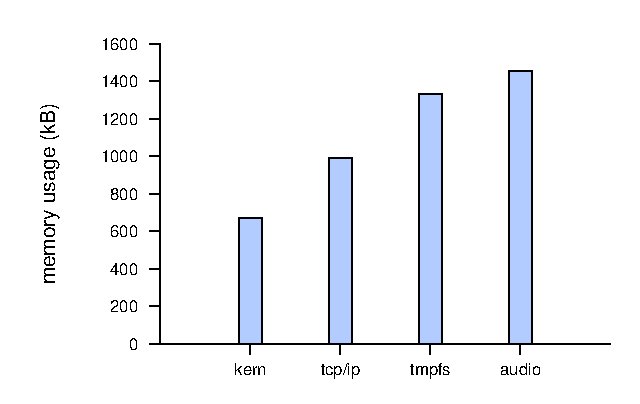
\includegraphics{memusage}
\caption[Memory usage of rump kernels per idle instance]{
\textbf{Memory usage of rump kernels per idle instance.}
The figures represent the amounts of memory used on the host.
}
\label{fig:memusage}
\end{figure}

Last, we look at performance figures for rump kernels.
Examples of the metrics include syscall overhead, memory footprint
and bootstrap time.  We compare results against other virtualization
technologies and against the native system.  Even though the anykernel
makes it possible to run the same drivers in the monolithic kernel as
well as rump kernels, the performance of a rump kernel needs to be on a
level where it does not hinder the execution of the intended use cases.
Furthermore, we are interested in seeing if rump kernels can outperform
other virtualization technologies.

\subsubsection{Memory Overhead}

We define memory overhead as the amount of memory required by the
virtualized OS.  We analyze the amount of memory required
to successfully boot a standard NetBSD installation up to the root
shell prompt in less than 5 minutes.  The results are
presented in Table~\ref{tab:minbootmem}.  They were obtained by
running \texttt{anita install} on the release build and testing if
the system boots with different values for \texttt{qemu -m}, where
the \texttt{-m} parameter controls the amount of hardware memory
presented to the guest.

A big difference between 5.1 and 5.99.48 is that the latter uses
a partially modular kernel by default.  Modularity means that all drivers
are not loaded at bootstrap, but rather on-demand as they are
required.  On-demand loading in turn means that the memory requirement of the
default installation of 5.99.48 is closer to what is actually
required by an application, since fewer unnecessary drivers
are loaded into unpageable kernel memory.  However, it is not
surprising that 5.99.48 requires more memory due to the tendency
of software to grow in size.

Still, the default installation may not represent the true minimum
required by an application.  If we estimate that the memory
consumption of NetBSD can be brought down to 1/4th by rigorous source level customization,
the true minimum memory required to boot the full OS version of
NetBSD 5.99.48 is 4.5MB.

Next, we present the \textit{host} memory consumption for various
rump kernel instances in Figure~\ref{fig:memusage}.  Again, we
measure the second instance for reasons listed above.  In the
figure, the \textit{kern} configuration contains nothing but the
rump kernel base.  The \textit{net} configuration contains TCP/IP
drivers.  The \textit{tmpfs} configuration supports mounting a tmpfs
file system, and the \textit{audio} configuration provides the
NetBSD pseudo-audio driver (\textit{pad}).  Notably, the audio
configuration also includes the vfs faction, since audio devices
are accessed via \texttt{/dev/audio}.

It needs to be stressed that Table~\ref{tab:minbootmem}
only measures the amount of memory used by the virtualized NetBSD
instance.  The true cost is the amount of memory used on the system
hosting the virtualized instance.  This cost includes the virtualization
container itself.  The memory consumption, ignoring disk cache,
for the \textit{second} \texttt{qemu~-n~24} instance for NetBSD~5.99.48
on the host is 38.2MB --- measuring the second instance avoids
one-off costs, which are not relevant when talking about scaling
capability.  The difference between what the guest uses and what
the host uses in this case is an additional 14.2MB in total memory
consumption.

When compared to the memory usage of 38.2MB for a virtual QEMU
instance, a rump kernel's default consumption is smaller by a factor of
more than 20.  This difference exists because a rump kernel does not need to
duplicate features which it borrows from the host, and due to its
flexible configurability, only the truly necessary set of components
is required in the guest.

\subsubsection{Bootstrap Time}

Startup time is important when the rump kernel is frequently
bootstrapped and ``thrown away''.  This transitory execution happens for example with
utilities and in test runs.  It is also an enjoyment factor with
interactive tasks, such as development work with a frequent iteration.
As we mentioned in Section~\ref{sect:conceptintro}, delays of over
100ms are perceivable to humans~\cite{miller:100ms}.

We measured the bootstrap times of a full NetBSD system for two setups, one on hardware and
one in a QEMU guest.  While bootstrap times can at least to some
degree be optimized by customization, the figures in
Table~\ref{tab:boottime} give us an indication of how long it takes to
boot NetBSD.  To put the figures into use case context, let
us think about the testing setup we mentioned in
Section~\ref{sect:testingstudies}.  The test suite boots 911 rump
kernels and an entire run takes 56~minutes.  Extrapolating from
Table~\ref{tab:boottime}, bootstrapping 911 instances of NetBSD in
QEMU takes 7.1 hours, which is seven and a half times as long as
running the entire test suite took using rump kernels.

The bootstrap times for various rump kernel faction configurations
are presented in Figure~\ref{fig:soloboot}.  In general, it can be
said that a rump kernel bootstraps itself in a matter of milliseconds,
\ie a rump kernel outperforms a full system by a factor of 1000 with
this metric.

\begin{table}[t]
\begin{tabular}{|l|l|l|l|}
\hline
platform & version & kernel boot & login prompt \\
\hline
\hline
hardware & NetBSD 5.1 & 8s & 22s \\
\hline
QEMU & NetBSD 5.99.48 & 14s & 28s \\
\hline
\end{tabular}
\caption[Bootstrap times for standard NetBSD installations]{
\textbf{Bootstrap times for standard NetBSD installations.}}
\label{tab:boottime}
\end{table}
\begin{figure}[t]
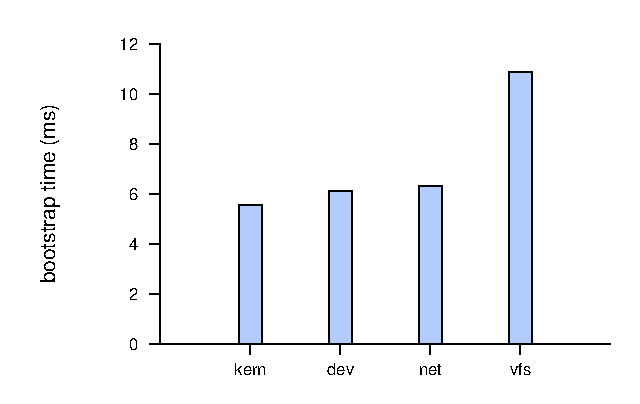
\includegraphics{soloboot}
\caption[Time required to bootstrap one rump kernel]{
\textbf{Time required to bootstrap one rump kernel.}
The time varies from configuration to configuration because of the
the initialization code that must be run during bootstrap.
}
\label{fig:soloboot}
\end{figure}

\subsubsection*{Network clusters}
\label{sect:netclust}

Bootstrapping a single node was measured to be an operation measured
in milliseconds.  High scalability and fast startup times make rump
kernel a promising option for large-scale networking
testing~\cite{hibler:emulab} by enabling physical hosts to have
multiple independent networking stacks and routing tables.

We measure the total time it takes to bootstrap, configure and send
an ICMP~ECHO packet through a networking cluster with up
to 255 instances of a rump kernel.  The purpose of the ICMP~ECHO
is to \textit{verify} that all nodes are functional.  The
cluster is of linear topology, where node $n$ can talk to
the neighboring $n-1$ and $n+1$.  This topology means that there are up to 254
hops in the network, from node $1$ to $255$.

We measured two different setups.  In the first one we used standard
binaries provided by a NetBSD installation to start and configure
the rump kernels acting as the nodes.  This remote client approach
is most likely the one that will be used by most for casual testing,
since it is simple and requires no coding or compiling.  We timed
the script shown in Figure~\ref{fig:testping.sh}.  In the second
setup we wrote a self-contained C program which bootstrapped a
TCP/IP stack and configured its interfaces and routing tables.
This local client approach is slightly more work to implement, but
can be used if node startup and configuration is a bottleneck.
Both approaches provide the same features during runtime.  The
results are presented in Figure~\ref{fig:clusterstart}.

\begin{figure}
{\tt \scriptsize
\begin{verbatim}
#!/bin/sh

RUMP_COMP='-lrumpnet -lrumpnet_net -lrumpnet_netinet -lrumpnet_shmif'
[ $# -ne 1 ] && echo 'need count' && exit 1
[ ! $1 -ge 3 -o ! $1 -le 255 ] && echo 'count between 3 and 255' && exit 1
tot=$1

startserver()
{
        net=${1}
        export RUMP_SERVER=unix://rumpnet${net}
        next=$((${net} + 1))
        rump_server ${RUMP_COMP} ${RUMP_SERVER}

        rump.ifconfig shmif0 create
        rump.ifconfig shmif0 linkstr shm/shmif${net}
        rump.ifconfig shmif0 inet 1.2.${net}.1 netmask 0xffffff00

        if [ ${net} -ne ${tot} ]; then
                rump.ifconfig shmif1 create
                rump.ifconfig shmif1 linkstr shm/shmif${next}
                rump.ifconfig shmif1 inet 1.2.${next}.2 netmask 0xffffff00
        fi

        [ ${net} -ne 1 ] && \
            rump.route add -net 1.2.1.0 -netmask 0xffffff00 1.2.${net}.2
        [ ${next} -ne ${tot} -a ${net} -ne ${tot} ] && \
            rump.route add -net 1.2.${tot}.0 -netmask 0xffffff00 1.2.${next}.1
}

for x in `jot ${tot}`; do
        startserver ${x}
done

env RUMP_SERVER=unix://rumpnet${tot} rump.ping -c 1 1.2.1.1
\end{verbatim}}
\caption[Script for starting, configuring and testing a network cluster]{
\textbf{Script for starting, configuring and testing a network cluster.}
This script can be used to test routing in up to the IP MAXTTL linearly
chained TCP/IP stacks.
}
\label{fig:testping.sh}
\end{figure}

\begin{figure}[t]
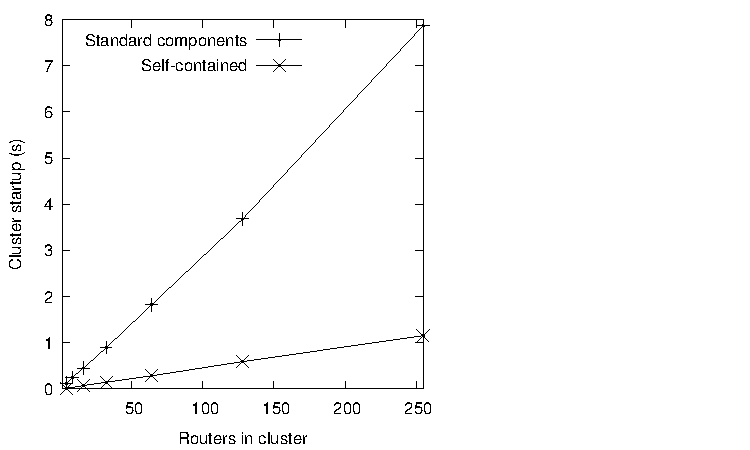
\includegraphics{clusterstart}
\caption[Time required to start, configure and send an initial packet]{
\textbf{Time required to start, configure and send an initial packet.}}
\label{fig:clusterstart}
\end{figure}

The standard component approach takes under 8s to start and configure
a networking cluster of 255 nodes.  Although this approach is fast enough
for most practical purposes, when testing clusters with 10-100x as
many nodes, this startup time can already constitute a noticeable delay in case
a full cluster is to be restarted.  Assuming linear scaling continues,
\ie hardware limits such as available memory are not hit, the local client approach can
bootstrap 10k nodes in 45 seconds, which is likely fast enough for
all cluster reboot purposes.

\subsubsection{System Call Speed}

We compared rump system call performance against other technologies:
Xen, QEMU (unaccelerated) and User-Mode Linux.  We did this comparison by
executing the \texttt{setrlimit()} system call 5 million times per
thread in two simultaneously running host threads.  We ran the UML
and Xen tests on a Linux host.  For calibration, we provide both
the NetBSD and Linux native cases.  We were unable to get UML or
QEMU to use more than one host CPU.  For a NetBSD host we present
native system calls, a rump kernel guest, and a QEMU NetBSD guest.
For Linux, we have native performance, a Linux Xen guest and a UML
guest.  The results are presented in Figure~\ref{fig:sandhoney}.
The NetBSD native call is 16\% faster than the Linux native call.
We use this ratio to normalize the results when comparing rump kernels
against Linux.  We did not investigate the reason for the difference
between NetBSD and Linux.

\begin{figure}
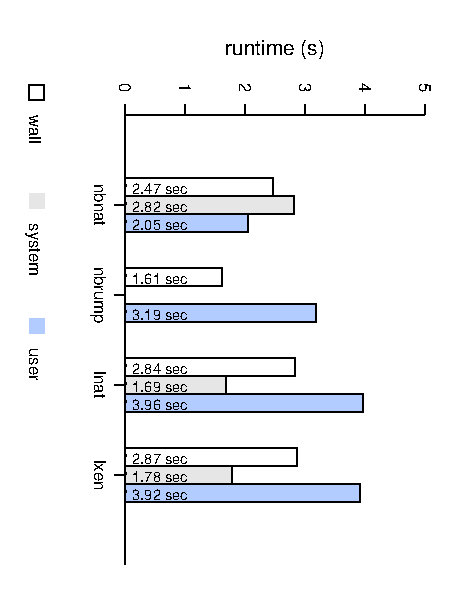
\includegraphics[angle=90]{syscall3}
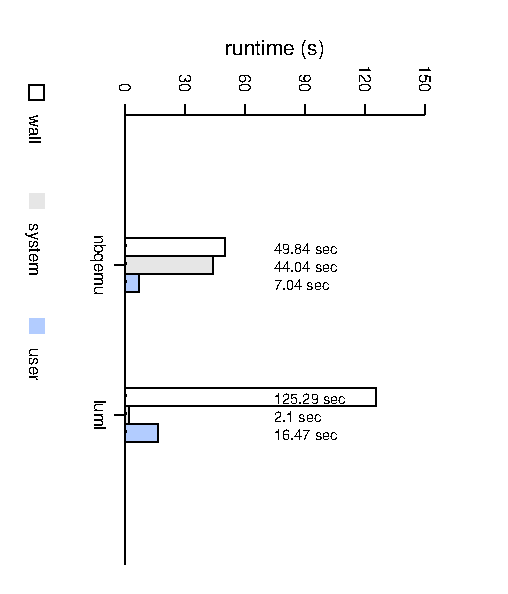
\includegraphics[angle=90]{syscall3-2}
\caption[Time to execute 5M system calls per thread in 2 parallel threads]{
\textbf{Time to execute 5M system calls per thread in 2 parallel threads.}
We divide the measurements into two figures since the durations are
vastly different.  The prefixes ``nb'' and ``l'' denote NetBSD and Linux
hosts, respectively.  As can be seen by comparing the user/system and
walls times in the first figure, the technologies measured there are
capable of using more than one host CPU.
Smaller wall times are better.
}
\label{fig:sandhoney}
\end{figure}
\clearpage

Rump kernel calls, as expected, carry the least overhead and are
the faster by over 50\% when compared to native system calls.  When
compared with the UML normalized performance, a rump kernel system
call performs 6707\% better.  We are unsure why UML performance is
this poor in wall time even though based on
literature~\cite{barham:xen,leslie:wombat} we expected it to be
significantly slower than a rump kernel.  QEMU performance is where
we expect it to be.

\subsubsection{Networking Latency}

To test packet transmission performance in virtual network cluster,
we used a linear setup like the one described in
Section~\ref{sect:netclust} and measure the time it takes for a
UDP packet to travel from one peer to another and back.  The results
as a function of the number of hops are displayed in Figure~\ref{fig:cluster}.
In the case of 255 nodes, the RTT translates to a 15.5$\mu$s
processing time per hop.

The cluster size we tested is limited by the maximum number of hops
that the IP time-to-live (TTL) field supports (255).  The recommended
default from RFC1340 is 64 hops, so we had to adjust the TTL to
255 manually (this adjustment was not an issue in Section~\ref{sect:netclust}, since
the ping utility does so automatically).

\begin{figure}[t]
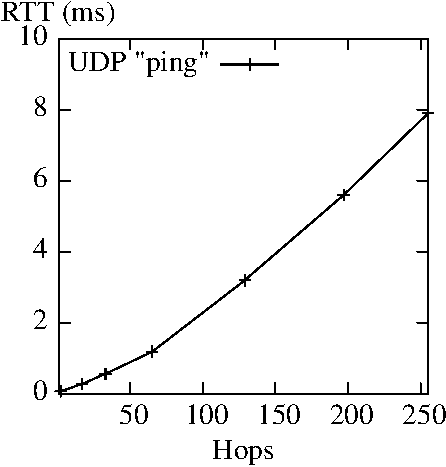
\includegraphics{latency.pdf}
\caption[UDP packet RTT]{
\textbf{UDP packet RTT.}
All rump kernel TCP/IP stacks are run on a single host.
}
\label{fig:cluster}
\end{figure}

\subsection{Summary}

We evaluated the anykernel architecture and rump kernels in numerous
different ways, both with synthetic benchmarks and analyzing real
world data from NetBSD collected between 2007 and 2011.

The use of rump kernels as an application library was evaluated
with file system related applications and was found to be a working
approach.  The \textit{makefs} application for NetBSD was reimplemented
as a local rump kernel client, and the new version was implemented
in under 1/17th of the time taken for the original.  This speedup
was due to the fact that the existing kernel file system driver
could be used directly.  The new version also supports four additional
file systems because driver support is available without further effort.

We evaluated the portability of the work in two ways.  First, we
tested running NetBSD rump kernels on foreign platforms.  While
support for portability is not complete, it works in practice
enough to run code.  Furthermore, we implemented prototypes
for Linux and FreeBSD, and found no reason to
suspect that a full implementation would not be possible.

Our security use case demonstrated that file system drivers running
inside the kernel are vulnerable to untrusted file system images.
A rump kernel running as a microkernel style server can be used to
isolate vulnerable kernel code into a separate domain when dealing
with untrusted images, and retain full in-kernel performance when
this isolation is not necessary.

There are close to a thousand tests that use rump kernels in daily
NetBSD test runs.  We looked at many different types of tests,
compared the implementation, result gathering and runtime overhead
with other possibilities for testing, and concluded that rump
kernels are superior for driver testing.  We also included examples
of what real-life regressions testing with rump kernels has enabled
to detect in NetBSD.

Finally, performance micro benchmarks confirmed that rump kernels
are lightweight and fast.  The memory overhead for a rump kernel
can be as low as 1/20th of that of a full kernel.  Bootstrapping
a rump kernel is 1,000 times faster than booting a full virtualized
kernel in QEMU.  We could boot a 255-node networking cluster with
255 virtualized TCP/IP stacks, configure all nodes and run an
initial roundtrip packet through them in 1.2 seconds.  System call
performance for local rump kernels is better than with any other
virtualization technology, and was measured to be 6707\% faster
than for example User-Mode Linux and 50\% faster than Xen.
